\documentclass[a4paper, 12pt]{article}
\usepackage[T2A]{fontenc}
\usepackage[utf8]{inputenc}
\usepackage[english,russian]{babel}
\usepackage{amsmath, amsfonts, amssymb, amsthm, mathtools, misccorr, indentfirst, multirow}
\begin{document}
	\begin{titlepage}
		\begin{center}
			\small
			МИНИСТЕРСТВО ОБРАЗОВАНИЯ И НАУКИ РОССИЙСКОЙ ФЕДЕРАЦИИ\\
			МОСКОВСКИЙ ФИЗИКО-ТЕХНИЧЕСКИЙ ИНСТИТУТ\\
			(ГОСУДАРСТВЕННЫЙ УНИВЕРСИТЕТ)\\
			\vspace{0.2cm}
			Кафедра вакуумной электроники\\
			\vspace{3cm}
			\large
			\textbf{Газоразрядный стабилизатор напряжения}\\
			\vspace{0.2cm}
			\small
			Лабораторная работа\\ по курсу \textit{Вакуумная электроника}\\
			\vspace{5cm}
			\begin{table}[h]
				\centering
				\begin{tabular}{cl}
					Составители: &Е.П Шешин,\\
					&А.В. Кудряшов,\\
					&Л.А. Кириченко
				\end{tabular}
			\end{table}
			\vspace{4.8cm}
			\small
			Москва\\МФТИ\\2018
		\end{center}
	\end{titlepage}
	\newpage
	УДК 621.387.1\\
	\vspace{0.2cm}
	
	\textbf{Газоразрядный стабилизатор напряжения: } лабораторная работа по курсу \textit{Вакуумная электроника} /сост.: Е.П. Шешин, А.В. Кудряшов, Л.А. Кириченко. — М.:МФТИ, 2015. – 32 с.\par
	\vspace{0.4cm}
	Описание лабораторной работы предназначено для студентов 2 курса, специализирующихся в области физической и вакуумной электроники.\par
	Работа предназначена для исследования газовых электрических разрядов в вакууме, которые кроме общефизического значения имеют большое практическое применение — от стабилизаторов напряжения до счетчиков элементарных частиц.\par
	\begin{flushright}
	\textbf{	УДК 621.387.1}\\
	\end{flushright}
	\pagenumbering{gobble}
	\newpage
	\pagenumbering{arabic}
	\tableofcontents
	\newpage
	\section{Введение. Цель работы}
	Газовым разрядом в широком смысле слова называется всякое прохождение электрического тока через газы.\par
	Газовые разряды бывают несамостоятельные и самостоятельные. Носители  тока в несамостоятельном разряде возникают за счет внешней ионизации (рентгеновское излучение, $\beta$- и $\gamma$-лучи и т.д.), не связанной с внешним напряжением, приложенным электродом газового промежутка. С прекращением ионизации такие разряды исчезают. Самостоятельные газовые разряды возникают в результате ионизации молекул и атомов самого газа, и их течение не зависит от внешней ионизации. Самостоятельный разряд — очень сложное явление, о чем свидетельствует даже просто перечисление его видов: тлеющий, дуговой, искровой, коронный и т. д.\par
	В данной работе подробно рассматривается в основном тлеющий разряд и основанное на его свойствах явление стабилизации напряжения (стабиловольта), а также ознакомиться с основными физическими явлениями, обуславливающими прохождение электрического тока в газах.
	\subsection{Электрический ток в газах}
Процессы токопрохождения в газах гораздо сложнее, чем в металлах, электролитах и проводниках. Напомним формулу для плотности какой-нибудь одной из составляющих общего тока (электронной, дырочной, ток положительных ионов, ток отрицательных ионов):
\begin{equation}
j=n_qqv
\end{equation}
где $n_q$ — концентрация частиц, $q$ — заряд частицы, $v$ — средняя скорость направления движения частиц к электроду.\par
Справедливость закона Ома для этих сред основано на том, что средняя скорость пропорциональна напряженности электрического поля $\mathbf{E}$:
\begin{equation}
\mathbf{v}=b\mathbf{E}
\end{equation}
где $b$ — коэффициент пропорциональности, называемый подвижностью, обычно зависящий от $\mathbf{E}$.\par
В металлах и электролитах концентрация носителей зарядов постоянна, и закон Ома верен. В полупроводниках концентрация экспоненциально растет с температурой, поэтому влияние джоулева тепла тока приводит к отклонению вольт-амперной характеристики, где увеличению тока $\Delta I$ соответствует уменьшение напряженности, вызванное уменьшением напряжения $\Delta U<0$. Подобное явление объясняется тем, что уменьшение подвижности зарядов компенсирует увеличение из концентрации. Такие участки называются участками с отрицательным дифференциальным сопротивлением $R_i$:
\begin{equation}
R_i=\frac{\Delta U}{\Delta I}<0
\end{equation}
\par
В газах концентрация носителей, из подвижность, напряженность поля могут сильно различаться не только в разрядах разного типа, но даже в различных участках самого разряда. Это является следствием множества факторов. Ведь из катода электрона могут попадать в межэлектродный промежуток вследствие различных видов эмиссии: термоэлектронной, автоэлектронной, бомбардировки катода положительными ионами разряда, фотоионизации излучением разряда. В самом межэлектродном промежутке заряженные частицы могут появляться вследствие инжекции их из других областей разряда, ионизации нейтральных молекул в результате столкновения с электронами, ионами, нейтральными молекулами (для высоких температур разряда), фотоэффекта, вызванного излучением самого разряда. В различных типах газового разряда преобладают различные процессы. Более того, в одном типе разряда в различных его частях проводимость газа обеспечивается различными процессами. Характер газового разряда зависит также от многих других факторов: от химической природы газа и электродов, от температуры и давления газа, от формы, размеров и взаимного расположения электродов, от напряжения, приложенного к электродам, от плотности тока и т.д. В силу всего этого вольт-амперная характеристика разряда имеет необычный вид, она не описывается законом Ома. Характеристика может быть неоднозначной функцией; одному и тому же значению напряжения на электродах может соответствовать несколько значений тока. Увеличение тока может быть вызвано не увеличением, а уменьшением напряжения и т.д.\par
Рассмотрение газового разряда начнем с простейшего несамостоятельного разряда между плоскими электродами.\par
Газы в нормальных условиях являются изоляторами, носители тока в них отсутствуют, точнее почти отсутствуют. Например в 1 см$^3$ ежесекундно под действием космических излучений и других причин рождается в среднем несколько пар ионов. Этот непрерывный процесс не приводит к заметной концентрации ионов, так как существует и другой непрерывный процесс — рекомбинация — нейтрализация разноименных ионов, положительных ионов и электронов. Устанавливается некоторая равновесная концентрация заряженных частиц, при которой скорости этих процессов равны. В воздухе эта концентрация порядка $10^3$ ионов в 1 см$^3$.\par
Такая концентрация слишком мала. Для сколь-нибудь заметной проводимости требуется большая концентрация, которая может возникнуть за счет инжекции (впрыскивания) заряженных частиц (ионов, электронов) в межэлектродный промежуток, ионизации нейтральных молекул газа каким-нибудь дополнительным внешним воздействием (нагреванием, облучением рентгеновским, ультрафиолетовыми лучами, радиоактивным излучением). Если проводимость газа исчезает с устранением внешнего воздействия, то такая проводимость называется \textbf{несамостоятельной}.\par
\begin{figure}[h]
\centering
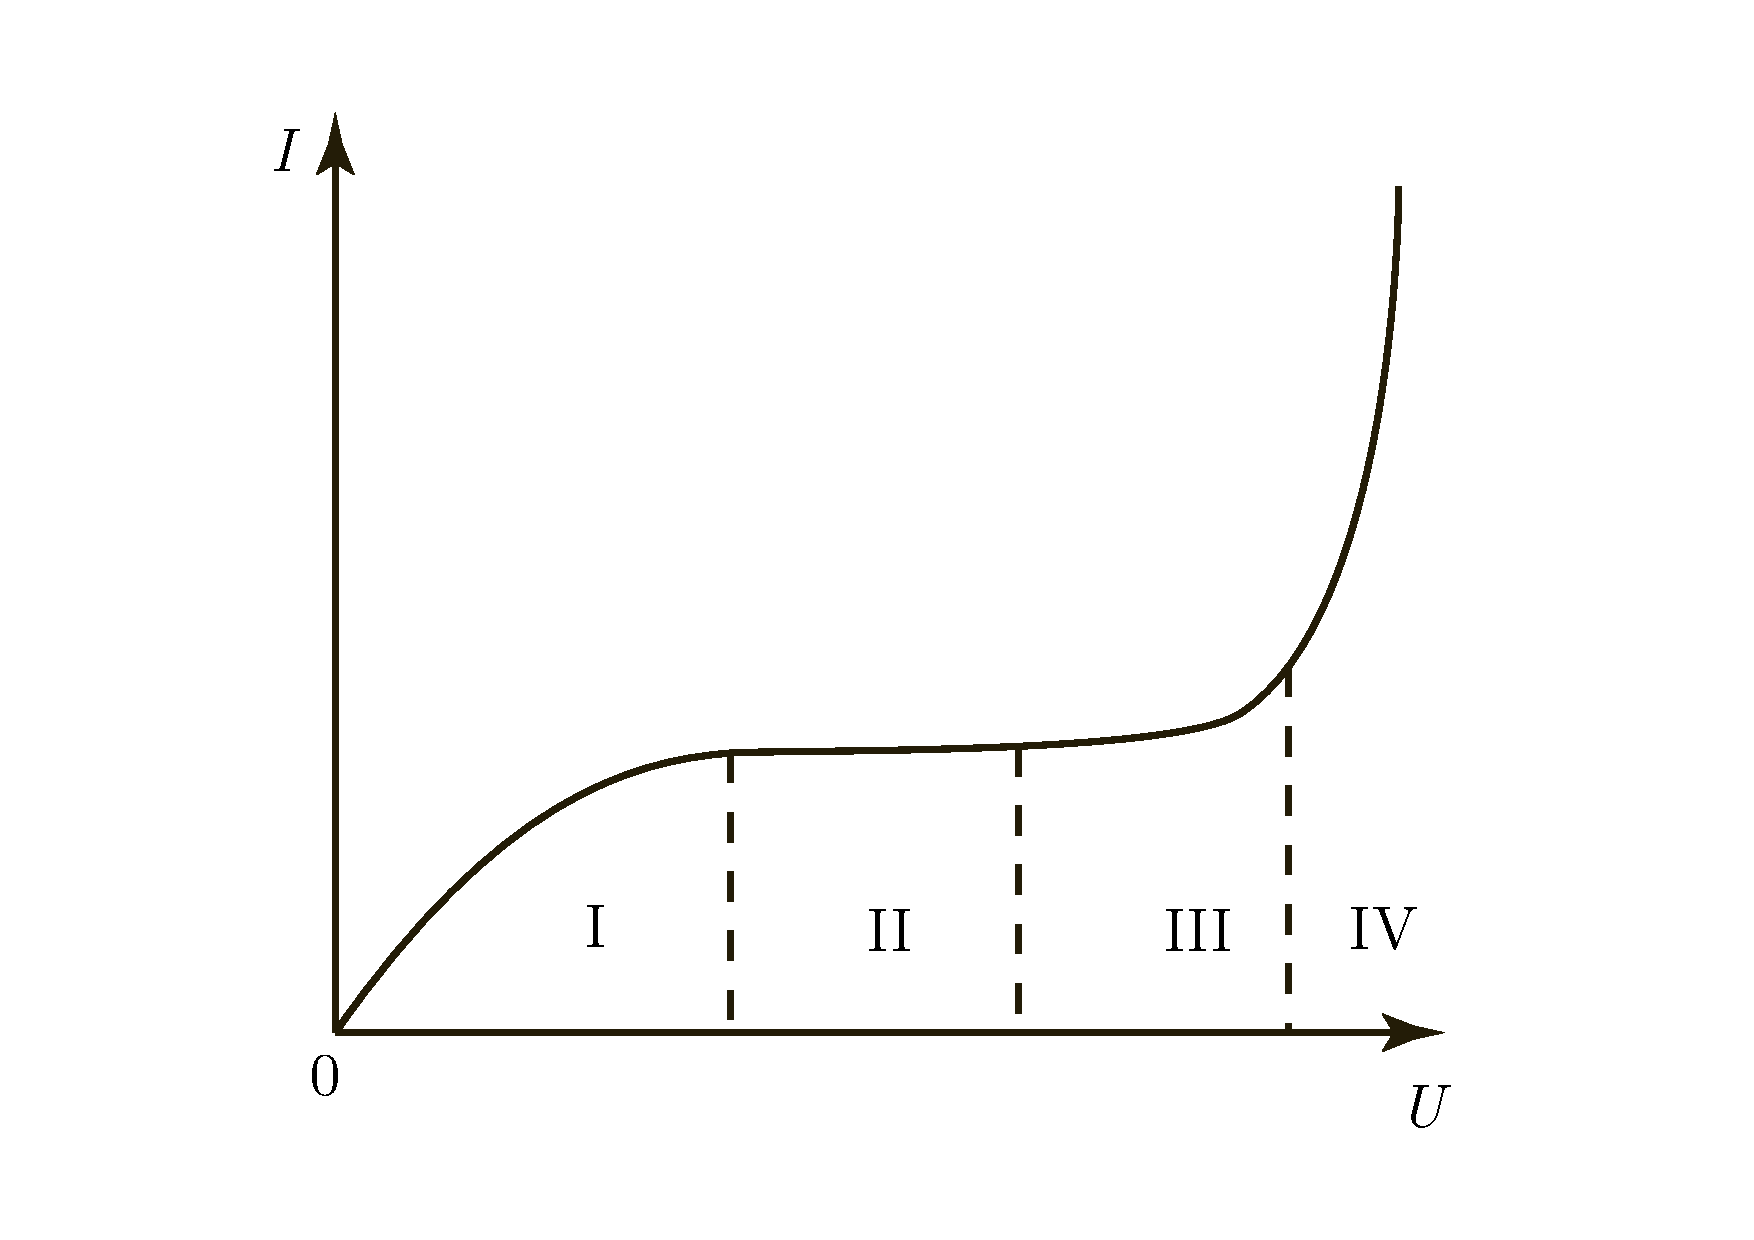
\includegraphics[scale=0.5]{Graph1.pdf}
\caption{Зависимость тока разряда от напряжения}
\label{fig:Graph1}
\end{figure}
На рис. \ref{fig:Graph1} изображена зависимость тока разряда от напряжения. На участке I ток растет с ростом напряжения (вначале линейно); на участке II ток остается постоянным; величина этого тока насыщения пропорциональна интенсивности внешнего ионизирующего фактора. Постоянство тока обозначает, что все родившиеся ионы достигают электродов, не успев прорекомбирировать. Ток насыщения ограничен ежесекундной генерацией ионов в межэлектродном промежутке. При дальнейшем увеличении напряжения ток вновь начинает расти (область III).\par
Рост тока вызван тем, что созданные внешним ионизатором заряженные частицы сами становятся способны вызывать ионизацию молекул за счет кинетической энергии, полученной ими при движении в электрическом поле. Этот режим называется режимом газового усиления. Участок IV соответствует переходу от несамостоятельного газового разряда к самостоятельному. Рассмотрим явления, соответствующие областям III и IV, более подробно. Хотя электроны и однозарядные ионы на одинаковом пути приобретают одинаковую энергию, главную роль в процессе ударной ионизации молекул играют электроны. Дело не только в том, что длина свободного пробега электронов больше длины свободного пробега ионов, главное в том, что чем меньше масса налетающей частицы, тем большую часть своей энергии частица может отдать молекуле при неупругом ударе, переводя её в возбужденное состояние или ионизируя. Зависимость вероятностей этих процессов от энергии элеткрона приведена на рис. \ref{fig:Graph2}.\par
\begin{figure}[h]
\centering
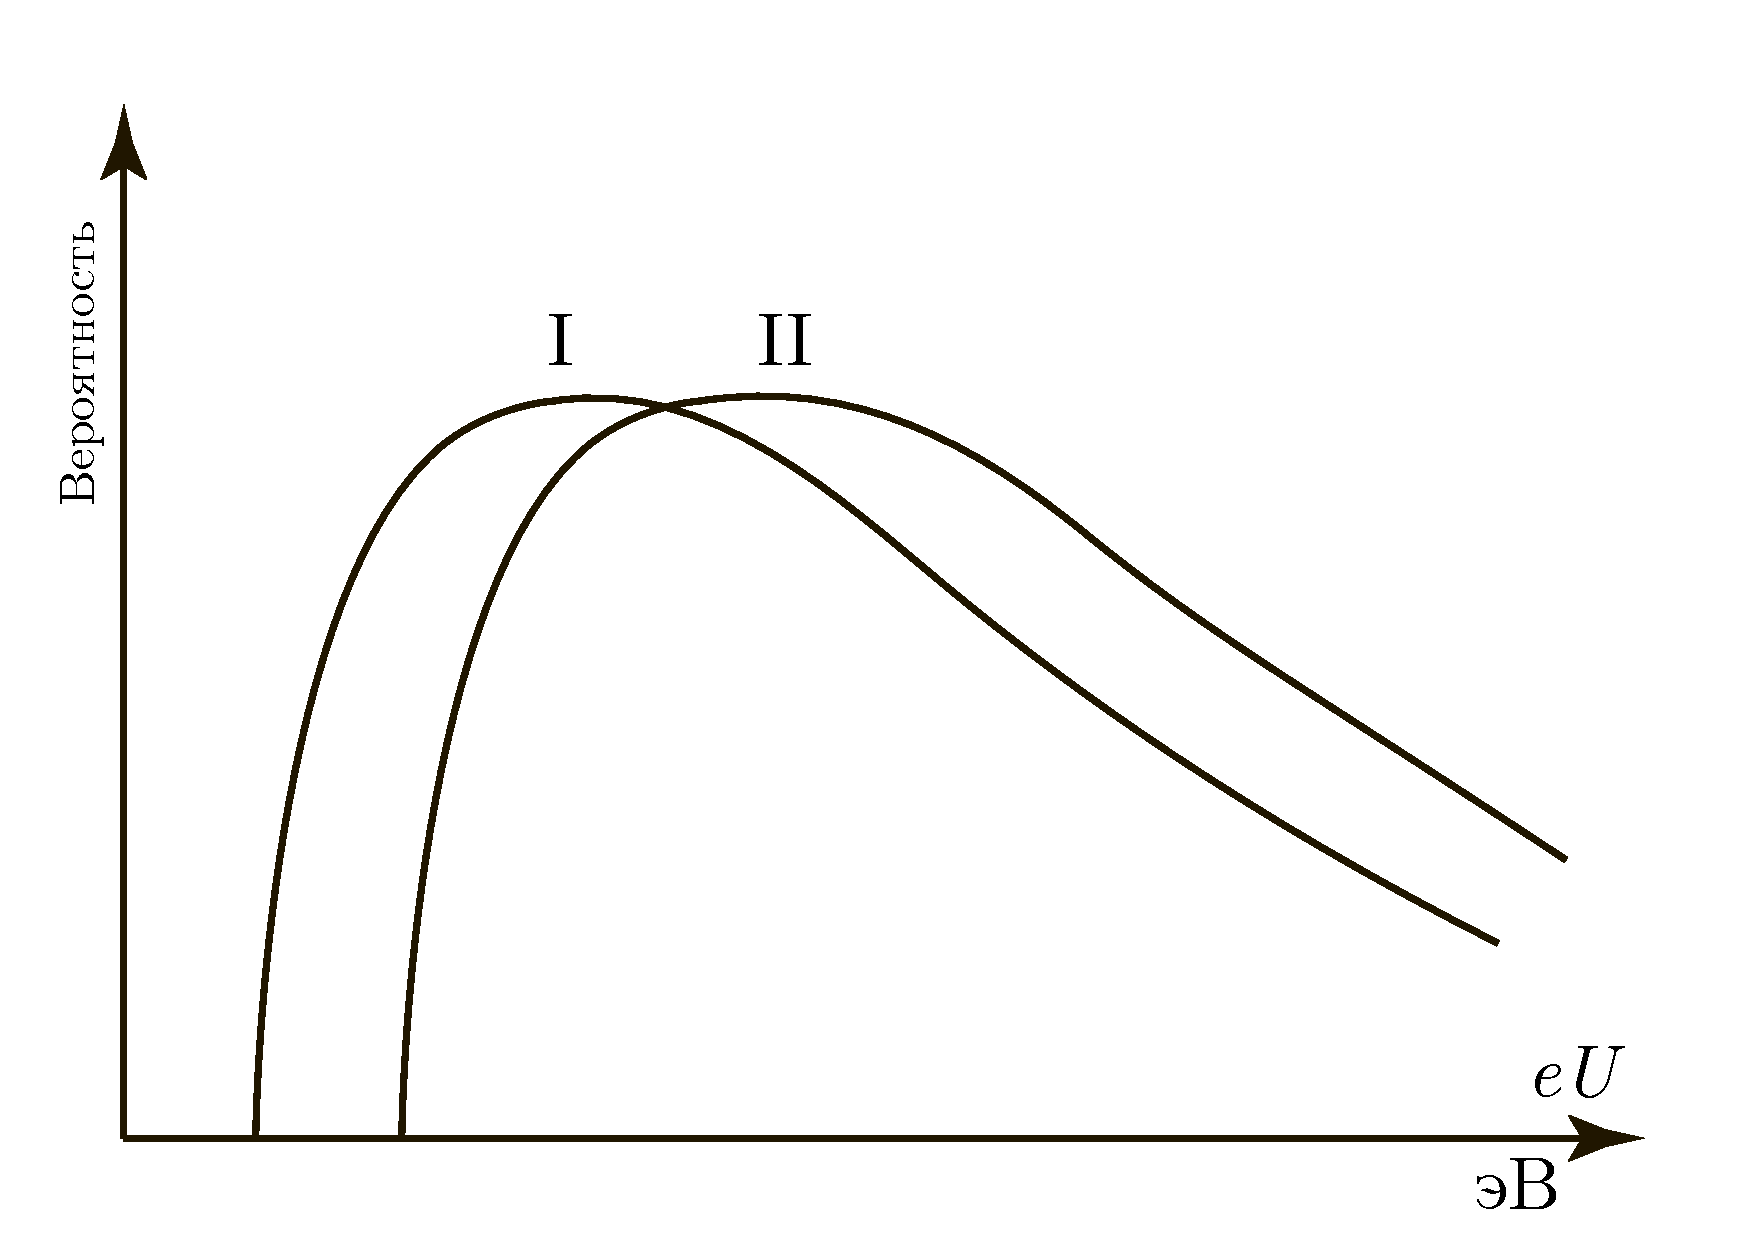
\includegraphics[scale = 0.4]{Graph2.pdf}
\caption{Зависимость вероятности процессов возбуждения и ионизации атомов от энергии налетающей частицы}
\label{fig:Graph2}
\end{figure}
Кривая I — вероятность процесса возбуждения, кривая II — ионизации. Поэтому в области III увеличение тока вызвано электронными лавинами: электрон ионизирует молекулу, уже два электрона ионизируют две молекулы и т.д.\par
Хотя величина полного тока одна и та же во всем межэлектродном промежутке, соотношения между электронной и ионной составляющими полного тока разряда различатся в разных его частях. Пусть электрон создает на единицу пути $\alpha$ электронов, тогда $n$ электронов, находящихся на расстоянии $x$ от катода, создадут на отрезке $dx$:
\begin{equation}
dn=n\alpha dx
\end{equation}
новых электронов. Если предположить, что от катода ежесекундно отходит $n_0$ электронов, возникших из-за внешнего источника ионизации, то на расстоянии $x$: от катода число электронов будет равно:
\begin{equation}
n_d=n_0e^{\alpha x}
\end{equation}
т.е. число электронов  экспоненциально возрастает. До анода, отстоящего от катода на расстояние $d$. дойдет
\begin{equation}
n_d=n_0e^{\alpha d}
\end{equation}
электронов. На рис. \ref{fig:Graph3} изображены величины электронных и ионных потоков в разряде.\par
\begin{figure}[h]
\centering
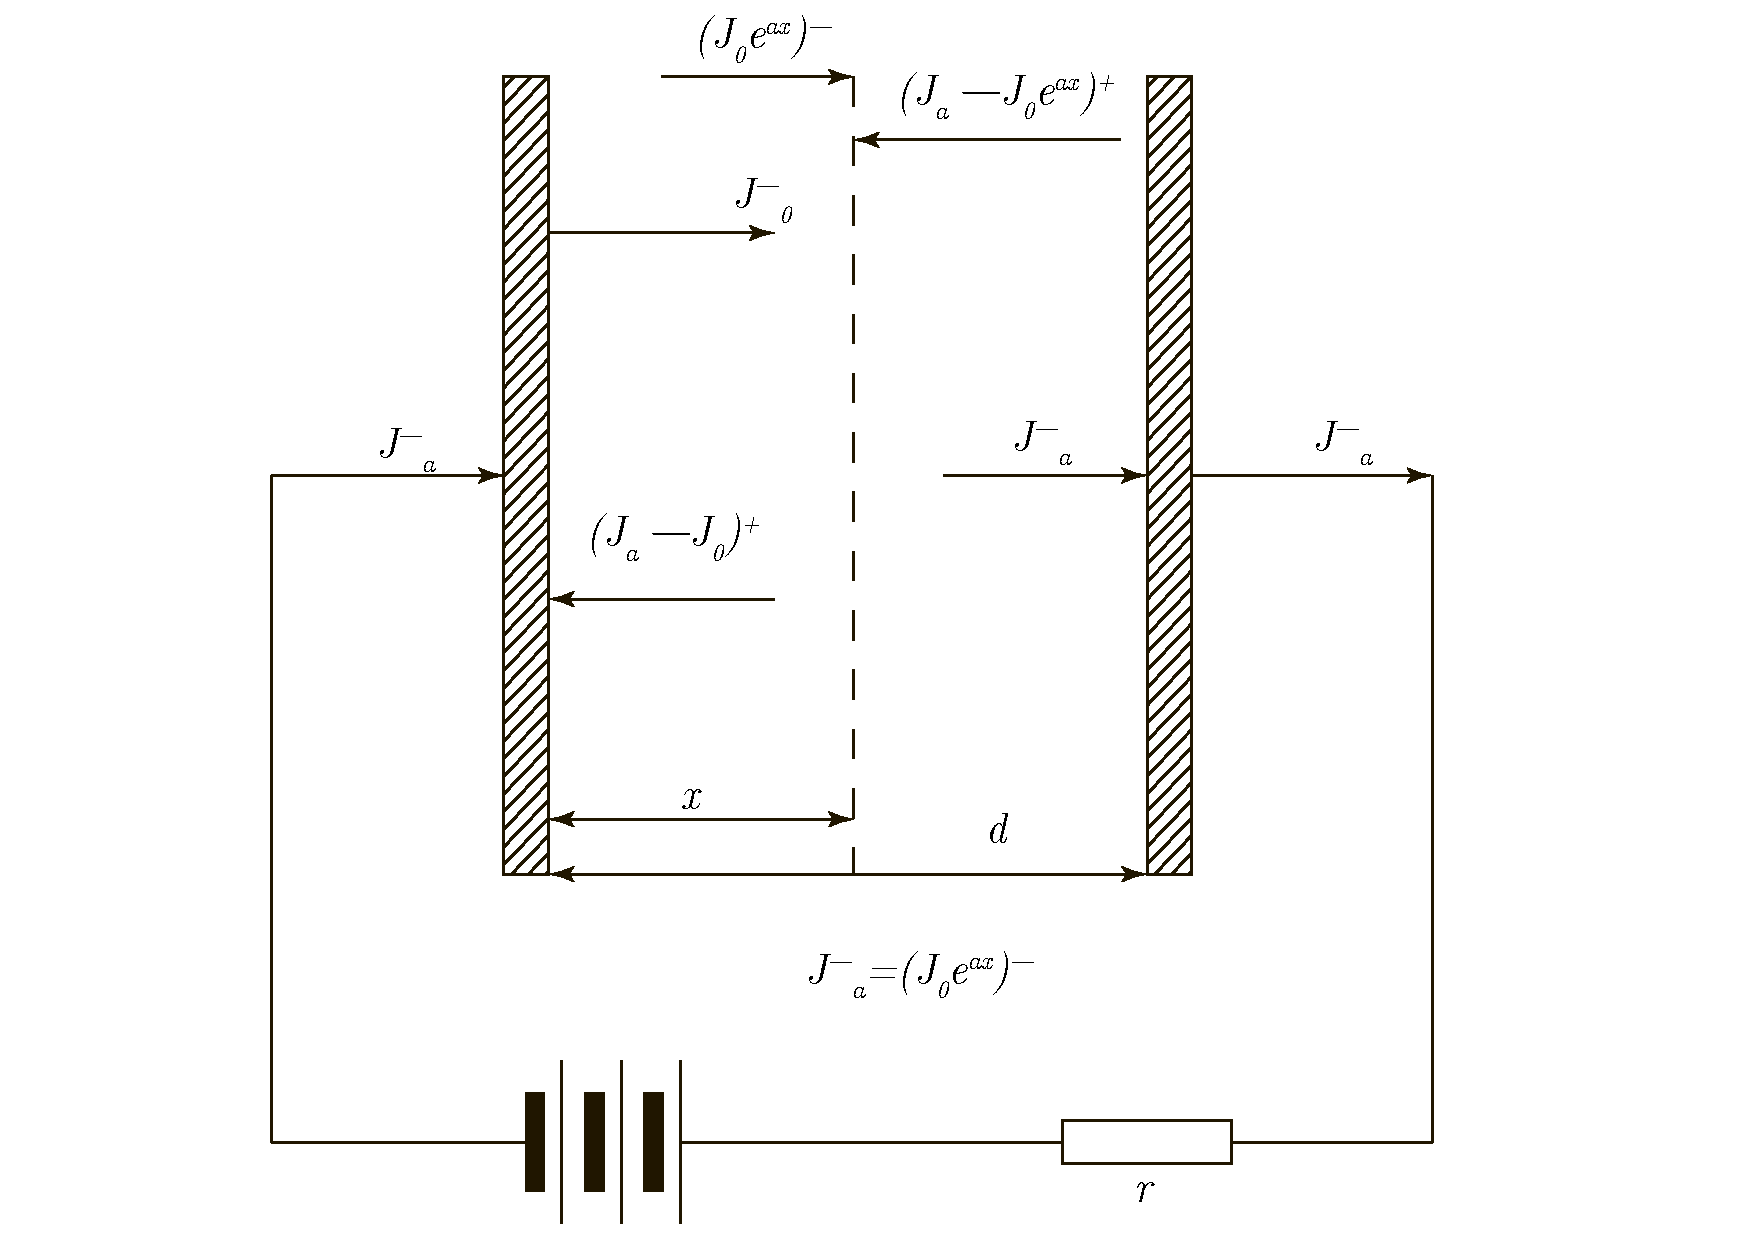
\includegraphics[scale=0.4]{Graph3.pdf}
\caption{Величины электронных и ионных потоков в разряде}
\label{fig:Graph3}
\end{figure}
Несмотря на усиление тока разряда по сравнению с током насыщения, которое может быть и тысячекратным, разряд остается несамостоятельным и прекращается, если устранить внешний источник ионизации. Лавины электронов дойдут до анода, а новых первичных электронов уже не будет. Если же положительные ионы приобретут энергию, достаточную для выбивания электронов из катода, то разряд может стать самостоятеьным. Выходящий из катода электрон приводит к созданию $e^{\alpha d}-1$ ионов. Эти ионы, достигая катода, выбивают из него электроны. Если обозначить $\gamma$ — среднее число электронов, выбитое одним ионом, то из катода будет выбито $\gamma\left(e^{\alpha d}-1\right)$ электронов. Если $\gamma\left(e^{\alpha d}-1\right)\ge 1$, то разряд оказывается самостоятельным. В случае знака "$>$" сила тока неограниченно возрастает, в случае же знака "$=$"  процесс протекает стационарно. Это условие пробоя (зажигания разряда). Коэффициент $\alpha$ пропорционален давлению газа и является функцией энергии электрона, полученной им от электрического поля на длине свободного пробега $\lambda$, которая обратно пропорциональна давлению:
\begin{equation}
\alpha=\rho f_1\left(\frac{E}{p}\right)
\end{equation}
где $E$ — напряженность электрического поля. Аналогично и коэффициент $\gamma$ можно записать в виде другой функции от того же аргумента:
\begin{equation}
\gamma=\rho f_2\left(\frac{E}{P}\right)
\end{equation}
\par
Учитывая, что непосредственно перед зажиганием разряда ток был невелик и объемный заряд не искажал распределения электрического поля, т.е. $E=E_3=\frac{U_3}{d}$, то условие возникновения самостоятельного разряда можно переписать в виде
\begin{equation}
f_2\left(\frac{U_3}{pd}\right)\left\{\exp\left[\frac{U_3}{pd}\right]-1\right\}=1
\end{equation}
\par
Это неявное выражение для зависимости напряжения зажигания $U_3$ лишь от произведения давления газа на расстояние между анодом и катодом, а не от каждого сомножителя в отдельности. Это частный случай закона подобия газовых разрядов. Графики этой зависимости для различных газов называются кривыми Пашена. Типичная кривая Пашена приведена на графике на рис. \ref{fig:Graph4}. При определенных значениях $\left(pd\right)_{\min}$ напряжение $U_3$ минимально. Этого напряжения недостаточно для зажигания разряда при уменьшении $pd$ относительно $\left(pd\right)_{\min}$, т.к. электронные лавины не успевают развиваться в необходимой мере при малых межэлектродных расстояниях и в условиях малой плотности газа. Поэтому зажигание разряда происходит при более высоком напряжении, чем $U_{3_{\min}}$. Аналогично, при больших значениях $pd>\left(pd\right)_{\min}$ увеличение напряжения зажигания связано, во-первых, с уменьшением напряженности поля при больших межэлектродных расстояниях и, во-вторых, с уменьшением длины свободного пробега электронов в условиях высокого давления (а следовательно, плотности) газа. Теперь лишь небольшая часть электронов успевает набрать между столкновениями с атомами энергию, достаточную для ионизации.\par
\begin{figure}
	\centering
	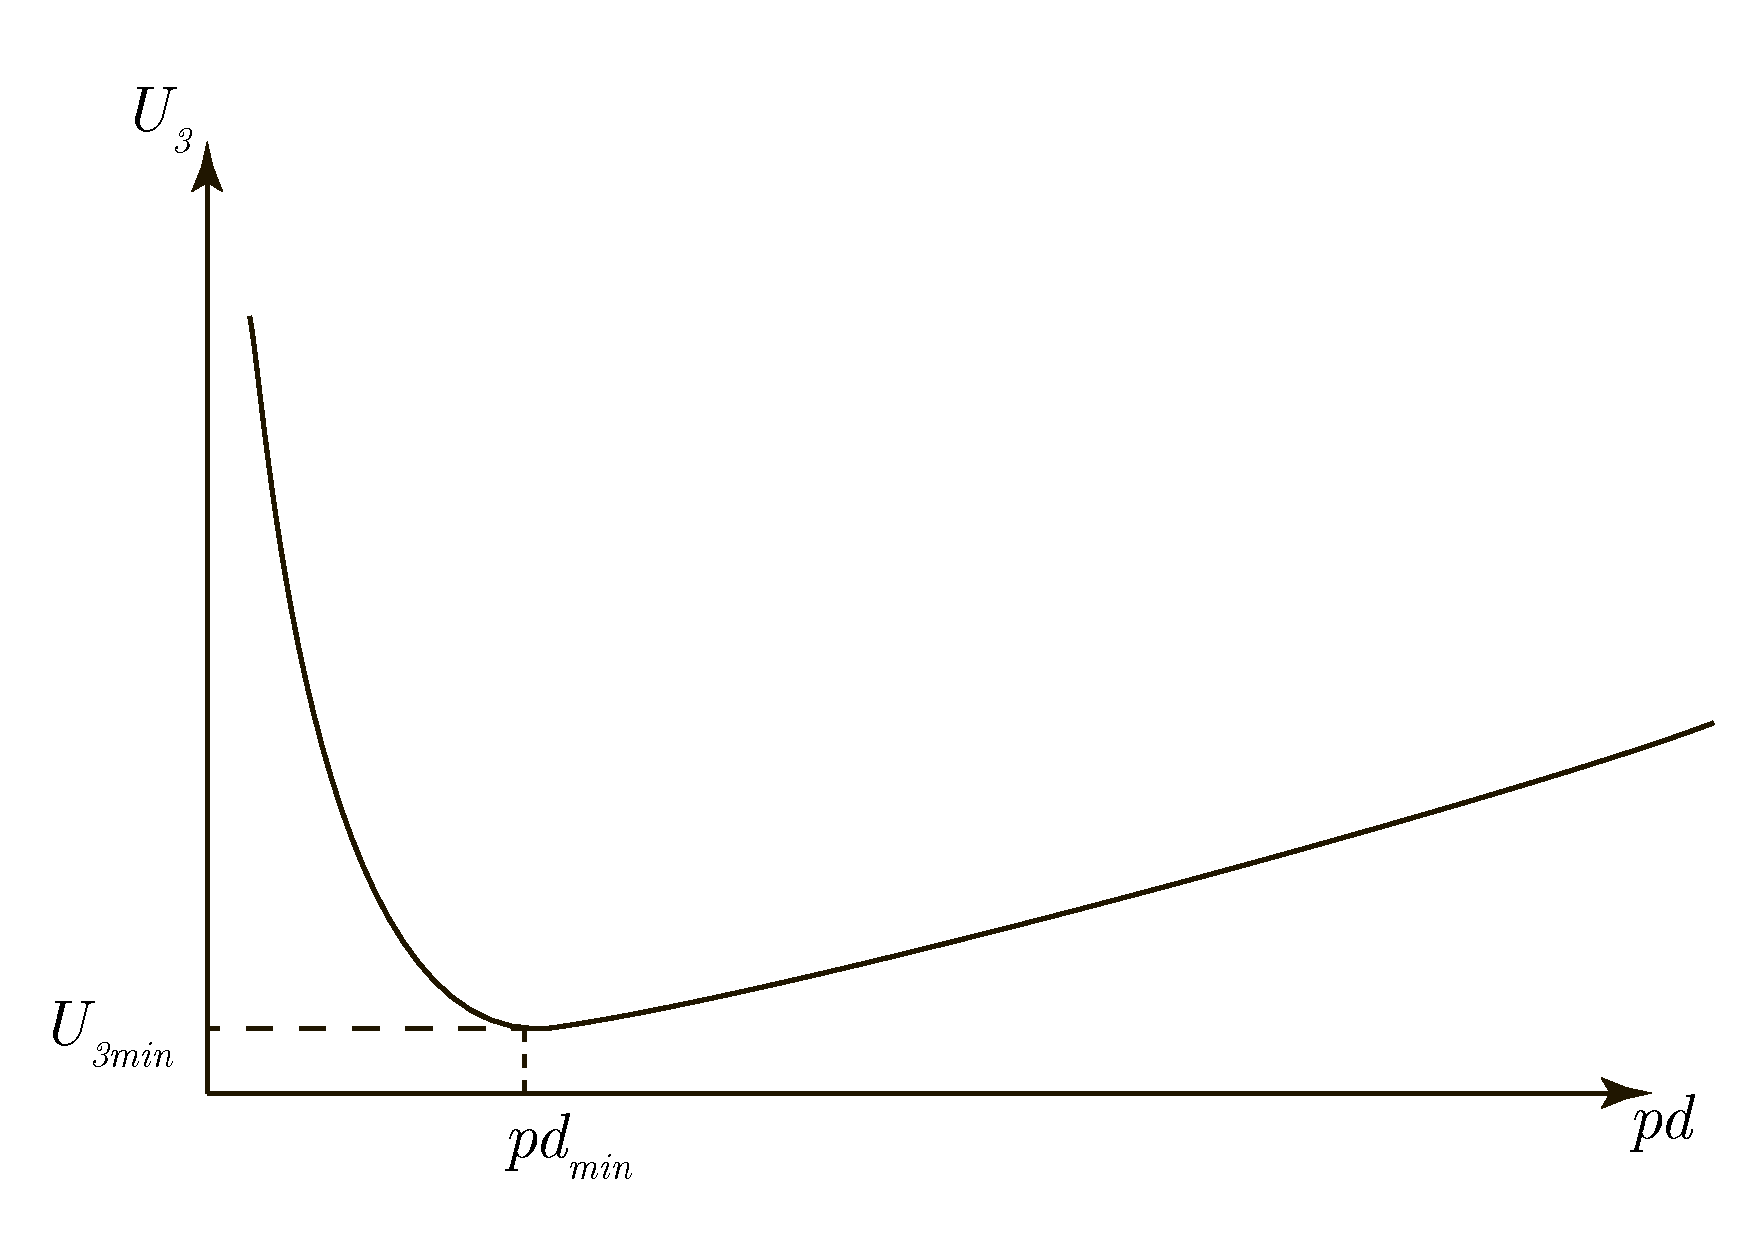
\includegraphics[scale=0.4]{Graph4.pdf}
	\caption{Типичная кривая Пашена}
	\label{fig:Graph4}
\end{figure}
	Отступление от закона Пашена наблюдается при больших давлениях, когда происходит искровой пробой разрядного промежутка, и при малых значениях $pd$, когда между электродами возникает вакуумный пробой с участием автоэлектронной эмиссии.\par
	На рис. \ref{fig:Graph5} изображена вольт-амперная характеристика прибора (газоразрядного диода) в широком диапазоне значений тока разряда, являющаяся продолжением графика на рис. \ref{fig:Graph1}. Участок I характеристики соответствует несамостоятельному разряду; 2 — несамостоятельному разряду, но с газовым усилением; 3 — соответствует переходу к тлеющему разряду; 4 — нормальному тлеющему разряду; 5 — аномальному тлеющему разряду; 6 — переходу разряда в дуговой; 7 — дуговому разряду, для которого характерна термоэмиссия электронов из раскаленного катода.\par
\begin{figure}[h]
	\centering
	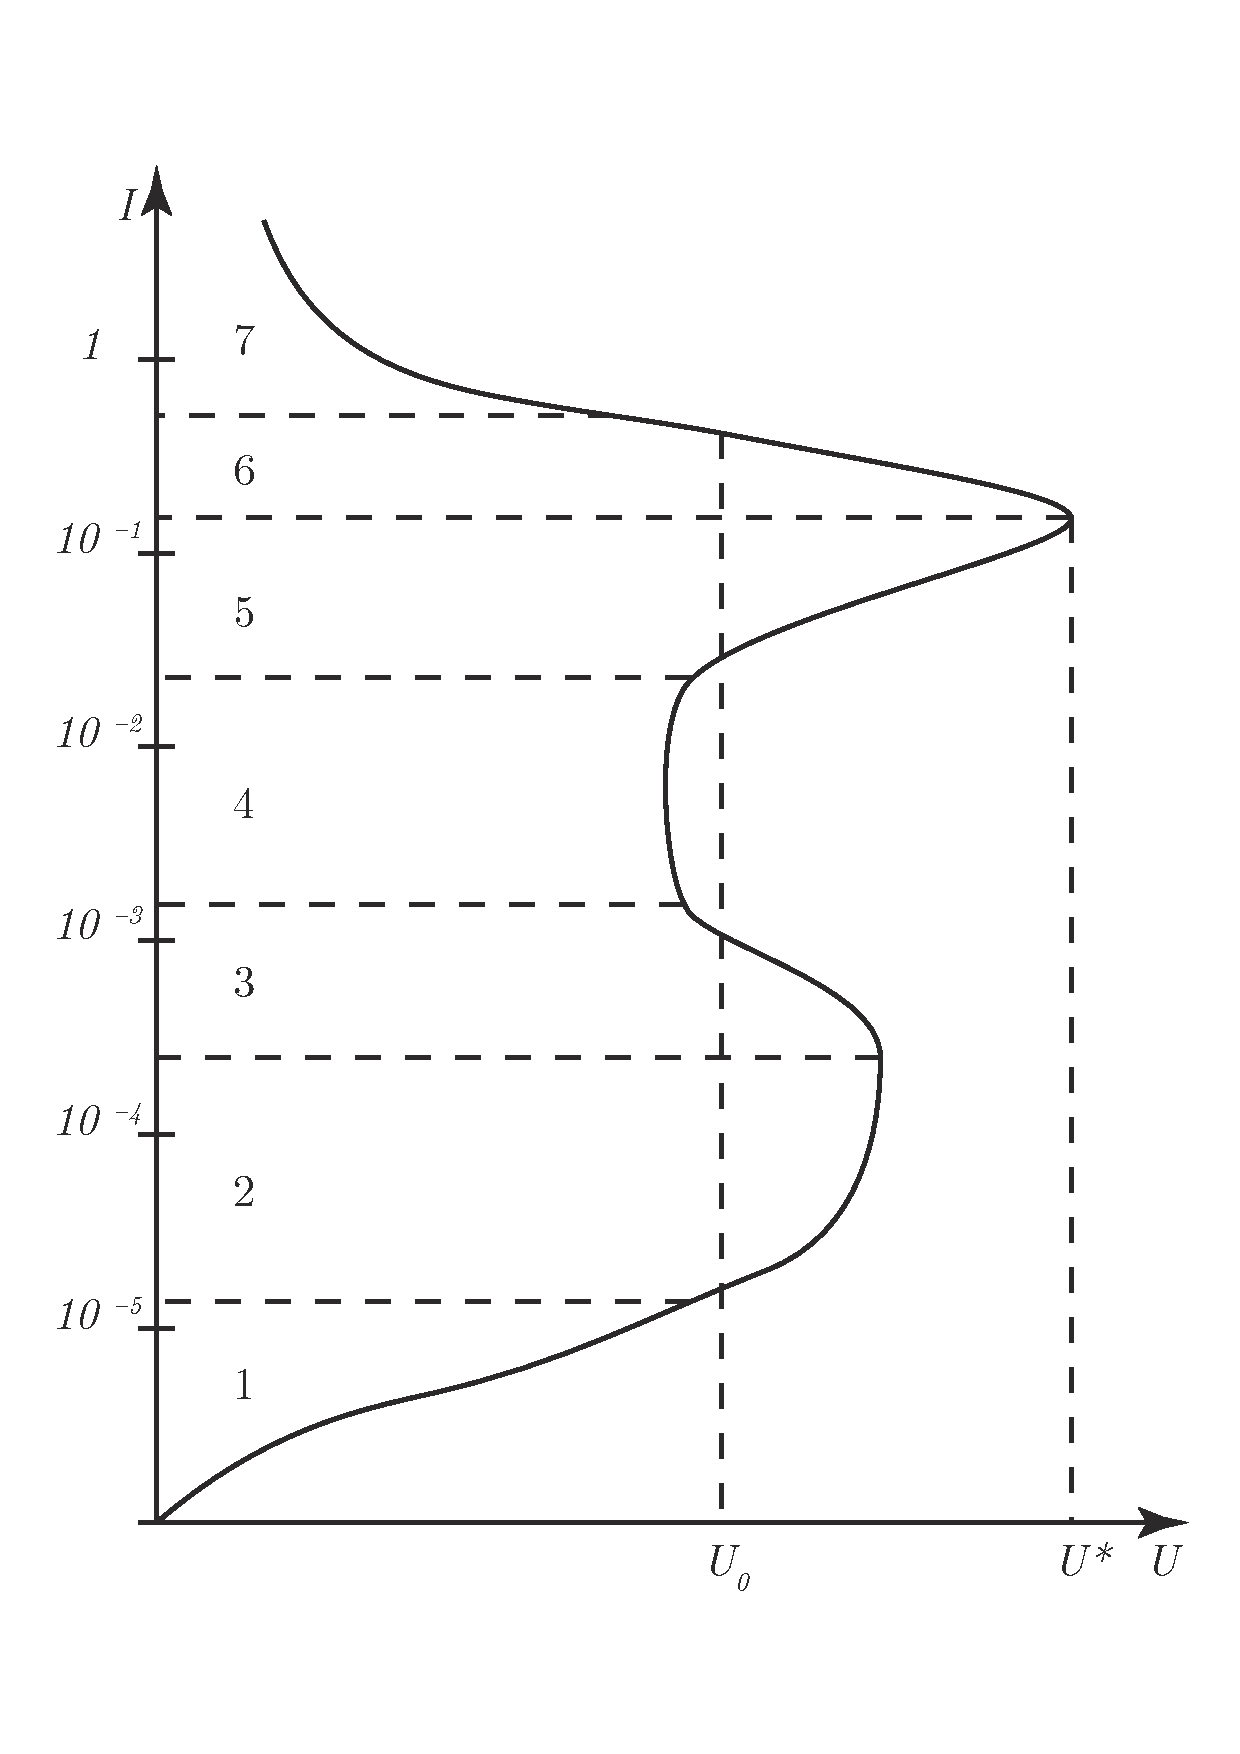
\includegraphics[scale=0.4]{Graph5.pdf}
	\caption{ВАХ газоразрядного диода в широком диапазоне значений тока разряда, являющаяся продолжением графика на рис \ref{fig:Graph1}}
	\label{fig:Graph5}
\end{figure}
	График на рис. \ref{fig:Graph5} довольно странен. Во-первых, напряжениям $U>U^*$ нет соответствующих значений тока. Значит ли это, что ток вообще не течет? Дело в том, что каждая точка кривой на рис. \ref{fig:Graph5} соответствует некоторому стационарному (способному существовать вечно) режиму газового разряда со своими значениями напряжения тока. В этих условиях существует равновесие трех процессов: генерация носителей заряда, их рекомбинация и их уходу на электроды.\par
	При напряжениях $U>U^*$ процесс генерации носителей преобладает над остальными двумя процессами. Поэтому проводимость газа и сила тока разряда непрерывно возрастают и изобразить этот процесс какой либо одной точкой на рис. \ref{fig:Graph5} невозможно. При этих напряжениях нет стационарных режимов газового разряда в данном приборе.\par
	Каждая стационарная точка кривой $J\left(U\right)$ может быть устойчивой или неустойчивой. Точка будет устойчивой, если малые отклонения от величин тока $J$ и напряжения разряда $U$ вызывают процессы, возвращающие ток и напряжение к их исходным значениям. И наоборот, стационарная точка будет неустойчивой, если малые отклонения тока и напряжения приводят к большим изменениям этих величин и возможному переходу разряда в новое стационарное состояние. Если увеличение концентрации носителей тока приводит к их дополнительной генерации, то точка характеристики неустойчива, если же увеличение концентрации носителей приводит лишь к росту скорости их рекомбинации, то ток разряда будет уменьшаться, возвращаясь к прежнему устойчивому своему значению.\par
	Во-вторых некоторым значениям напряжения на графике, например $U=U_0$, соответствуют несколько (до четырех) значений тока. Конечно в действительности всегда реализуется какое-то одно значение тока. Важную роль в том, какое значение тока будет реализовано, играет внешнее сопротивление $r$ на рис. \ref{fig:Graph8}. Ясно, что ток в разряде не может быть больше чем $\frac{\varepsilon}{r}$. Для нахождения тока разряда при заданной ЭДС источника $\varepsilon$ (которое можно изменять) при заданном сопротивлении $r$ (которое также может быть переменным) удобно воспользоваться графическим методом. Идея его основана на простом соотношении:
	\begin{equation}
		\varepsilon=U_p+Ir
	\end{equation}
	где $U_p$ — напряжение разряда. Если переписать это уравнение иначе
	\begin{equation}
		U_p=\varepsilon-Ir
	\end{equation}
	\par
	Пересечение графиков  левой части последнего уравнения и правой части даст искомую точку — напряжение разряда $U_p$ и ток разряда $J$. Для того, чтобы график правой части был предельно простым, и ток, и напряжение надо изображать не в логарифмическом, а в естественном линейном масштабе. В этом масштабе график правой части — прямая, называемая нагрузочной прямой.\par
	Неустойчивость некоторых участков вольтамперной характеристики и её последствия можно понять на обобщенном примере.\par
	На рис. \ref{fig:Graph6} изображена вольтамперная характеристика так называемого S-типа, на ней изображены несколько нагрузочных прямых, соответствующих ЭДС источника и одному и тому же внешнему сопротивлению $r$. Точками обозначены решения, соответствующие ЭДС $\varepsilon_1$, $\varepsilon_2$, $\varepsilon_3$, $\varepsilon_4$.
	\begin{figure}[h]
		\centering
		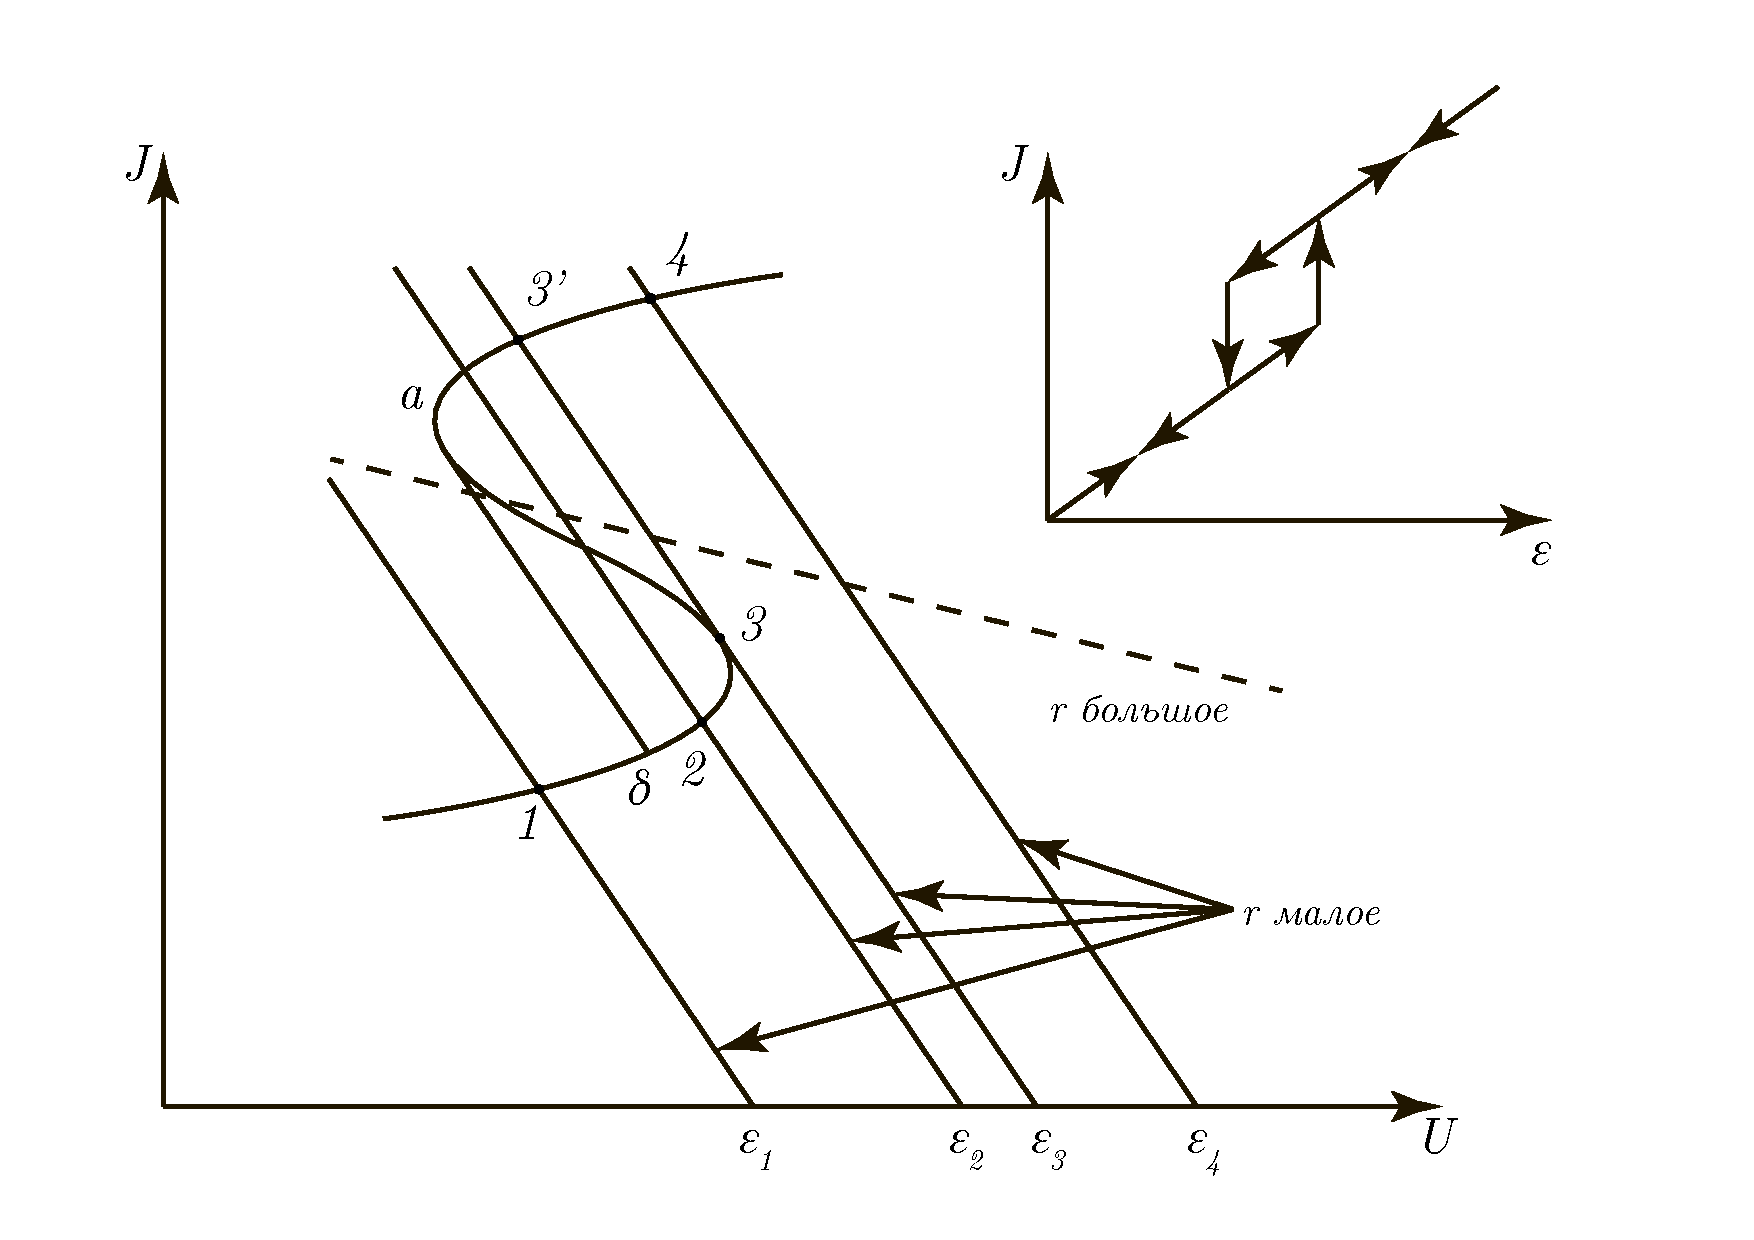
\includegraphics[scale=0.4]{Graph6.pdf}
		\caption{ВАХ S-типа}
		\label{fig:Graph6}
	\end{figure}
	\par
	При увеличении ЭДС от $\varepsilon_1$ до $\varepsilon_2$ ток разряда непрерывно увеличивается, переходя от точки 1 к точке 3. В окрестности точки 3 происходит лавинообразное увеличение проводимости газа, и точка, характеризующая состояние газового разряда, скачком перемещается по нагрузочной прямой в точку 3, где может существовать стационарное значение тока разряда. При дальнейшем росте ЭДС до $\varepsilon_4$ происходит непрерывный рост тока от точки 3 до точки 4.\par
	Если начать уменьшать ЭДС источника, ток будет непрерывно уменьшаться до точки $a$, потом скачком уменьшится до точки $\delta$, а потом будет плавно уменьшаться до нуля. На вставке к рис. \ref{fig:Graph6} изображена зависимость тока разряда от ЭДС источника. Такой ход характеристики называется гистерезисом разряда.\par
	Из графика ясно, что если нагрузочная прямая очень пологая (изображена пунктиром), то она пересекает вольт-амперную характеристику только в одной точке. Это соответствует большому внешнему сопротивлению $r$ большое и большому напряжению источника. Условием этого является:
	\begin{equation}
		r>\left|R_i\right|
	\end{equation}
	где $R_i=\frac{dU}{dI}$ — дифференциальное сопротивление разряда, которое может быть и отрицательным (на участке между точками $a$ и 3).\par
	Рассмотрим основные особенности тлеющего разряда. Переход от несамостоятельного разряда к самостоятельному обычно сопровождается резким увеличением силы тока и внезапным появлением течения газа. Однако если внешнее сопротивление очень велико (порядка 106 Ом), переход от несамостоятельного разряда к самостоятельному совершается постепенно, и можно наблюдать переходную форму разряда. При напряжении, равном напряжению зажигания, около анода появляется слабое свечение. Если плотность тока лежит в пределах $10^{-15}-10^{-6}$ А/см$^2$, создаваемый им объемным зарядом можно пренебречь. При увеличении тока начинается искажение поля пространственными зарядами, а свечение начинает распространяться по направлению к катоду. При дальнейшем увеличении силы тока свечение газа начинает распадаться на характерные для тлеющего разряда части, а падение потенциала в трубке сосредоточивается в катодных частях разряда. Обычно тлеющий разряд возникает при низких давлениях (от сотых долей до десятков мм рт. ст.).\par
	В тлеющем разряде можно различить несколько чередующихся областей с различно протекающими процессами возбуждения, ионизации и рекомбинации зарядов. Все эти области можно наблюдать по различной интенсивности свечения газа лишь в достаточно длинной трубке, где анод и катод удалены на десятки сантиметров. Для полноты описания тлеющего разряда кратко опишем все области, хотя в данной работе можно наблюдать лишь часть из них, расположенных у катода.\par
	На рис. \ref{fig:Graph7} изображены области тлеющего разряда и распределение потенциала в газоразрядной трубке. Физика явлений, происходящих в различных областях тлеющего разряда. Физика явлений, происходящих в различных областях тлеющего разряда, может быть качественно описана следующим образом (номера областей соответствуют номерам на рис. \ref{fig:Graph7}). Светящиеся области разряда заштрихованы.\par
	\begin{figure}[h]
		\centering
		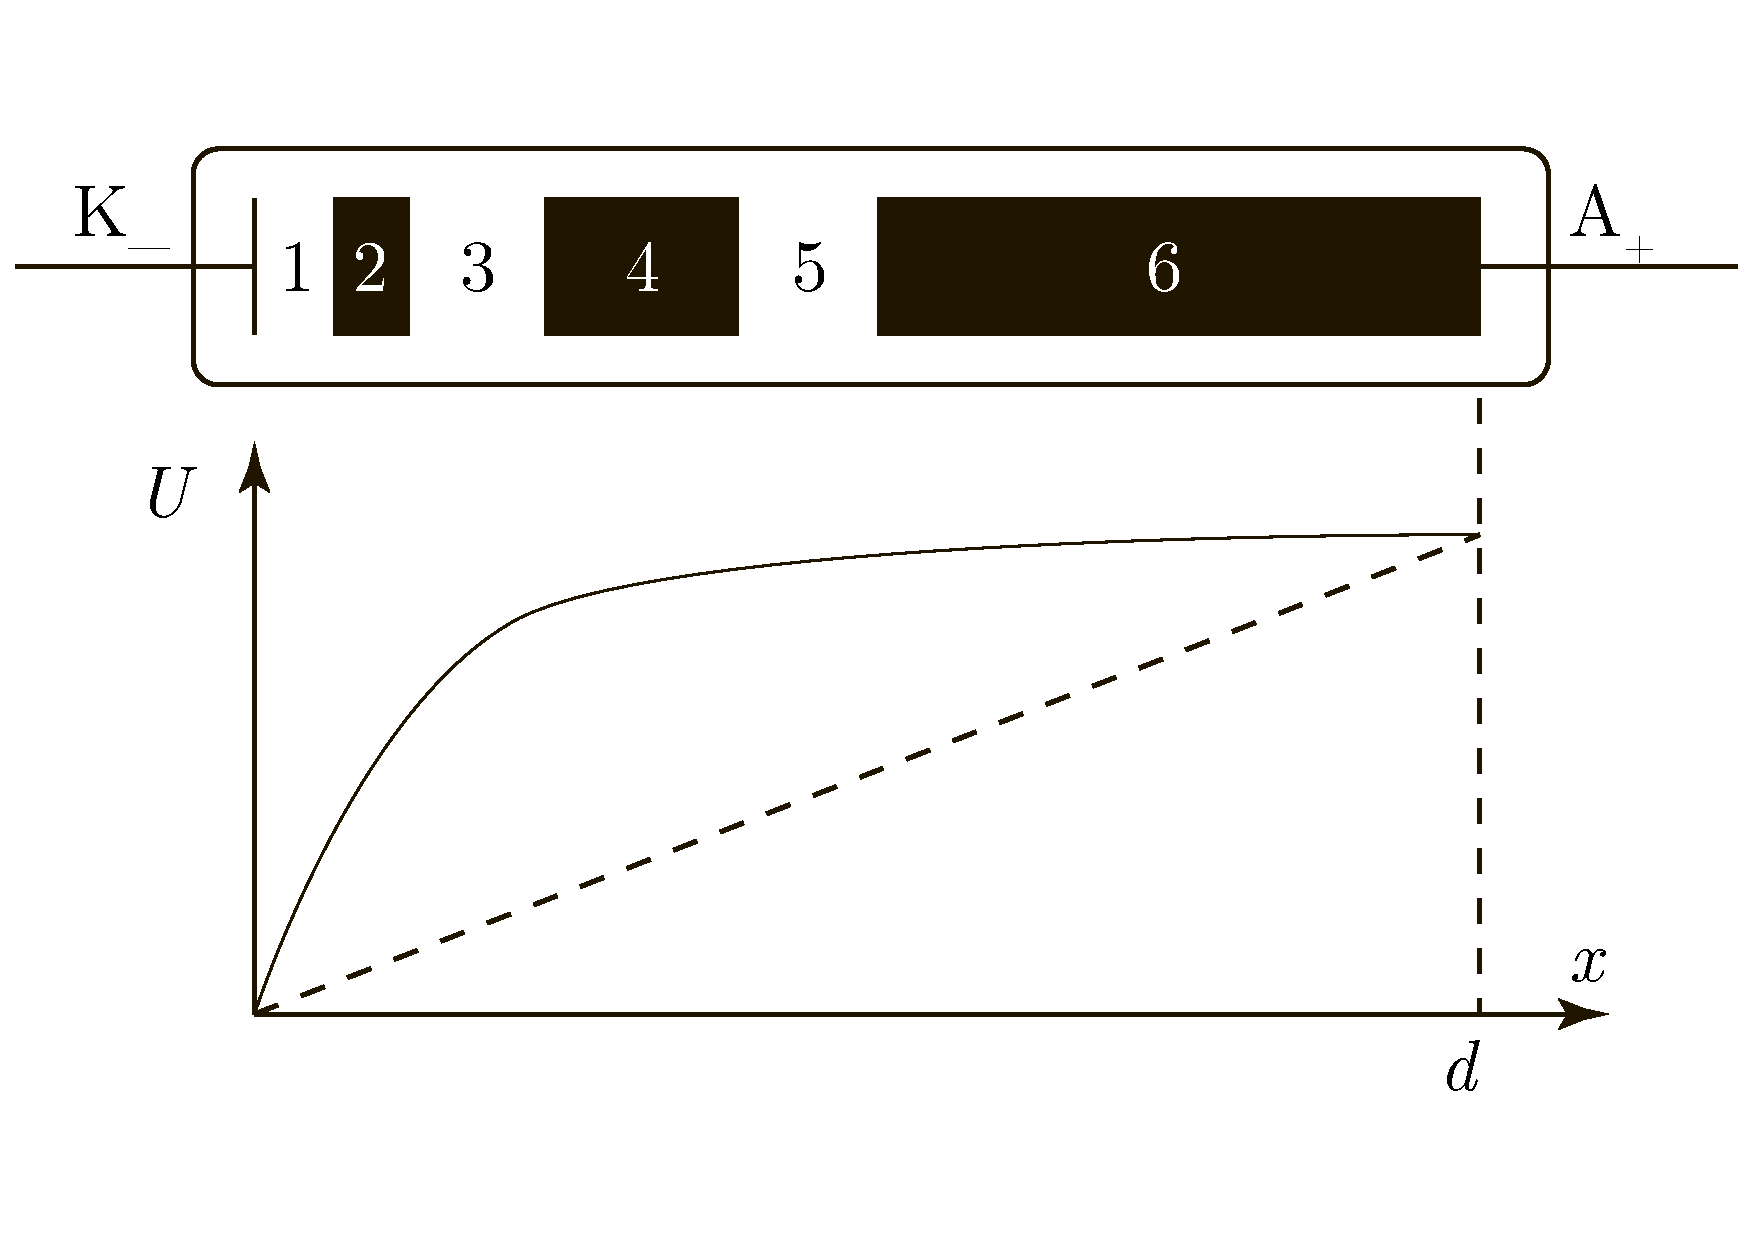
\includegraphics[scale=0.4]{Graph7.pdf}
		\caption{Области тлеющего разряда и распределение потенциала в газоразрядной трубке}
		\label{fig:Graph7}
	\end{figure}
	\textit{Название областей:}
	\begin{enumerate}
		\item астоново темное пространство;
		\item катодная светящаяся пленка;
		\item катодное темное пространство;
		\item тлеющее свечение;
		\item темное фарадеево пространство;
		\item область положительного столба (плазма)
	\end{enumerate}
	\par
	Рассмотрим характерные свойства указанных областей тлеющего заряда.
	\begin{enumerate}
		\item Астоново темное пространство (десятые доли мм) — область, где энергия выбитых из катодов электронов еще недостаточна ни для возбуждения, ни для ионизации. Свечение отсутствует.
		\item Катодня светящаяся пленка обязана тому, что электроны уже достигли энергии возбуждения молекул, что приводит к последующему излучению света. Для ионизации энергия электронов недостаточна.
		\item В этой области начинаются электронные лавины, так как сюда дошедшие без столкновений электроны уже обладают энергией, достаточной для ионизации молекул. Созданные положительные ионы обеспечивают необходимую эмиссию электронов из катода. В этой области преобладает положительный объемный заряд. Интенсивность свечения уменьшается, так как вероятность возбуждения при этих энергиях электронов мала. Рекомбинация же ионов и электронов маловероятна из-за их большой относительной скорости.\par
		На первые три области приходится основное падение потенциала, называемое катодным падением потенциала. Развивающиеся электронные лавины создают высокую степень ионизации газа, поэтому проводимость остальных участков разряда значительно выше, чем в областях катодного падения потенциала, поэтому изменение потенциала в них невелико.
		\item В этой области высока концентрация электронов и ионов. Тлеющее свечение является следствием их рекомбинации. Интенсивная рекомбинация приводит к уменьшению концентрации электронов и ионов.
		\item В темном фарадеевском пространстве концентрация заряженных частиц уже меньше, чем в области 4, поэтому вероятность рекомбинации и интенсивность свечения падают. Оставшиеся свободные носители тока, ускоряясь, вызывают ионизацию и возбуждение молекул газа.
		\item Переход таких молекул в нормальное состояние сопровождается свечением, характерным для анодного (положительного) столба разряда, который представляет собой газоразрядную плазму (с суммарным зарядом, близким к нулю и высокой концентрацией заряженных частиц). Свечение вызвано переходами возбужденных молекул в основное состояние.
	\end{enumerate}
	\par
	Какая часть заряда играет большую роль? Опыт показывает, что при уменьшении расстояния между электродами катодные части разряда сохраняются всегда неизменными, в то время, как длина положительного столба уменьшается до его полного исчезновения. Наиболее важной является область катодного падения (области 1, 2, 3), а положительный столб служит для передачи тока через газ.\par
	Вернемся к рис. \ref{fig:Graph5}. На нем участок графика 3 — переход к тлеющему разряду. Рост силы разрядного тока на этом участке происходит даже при уменьшении напряжения разряда. Это является демонстрацией эффекта сокращения протяженности области прикатодного пространства вследствие появления объемного положительного заряда. Из рис. \ref{fig:Graph7} следует, что появление вблизи катода положительного объемного заряда увеличивает напряженность поля, которая заметно превышает первоначальное её значение (соответствующее ей распределение потенциала изображено пунктиром). В результате необходимая для развития лавин напряженность поля поддерживается при напряжениях, меньших, чем первоначальное напряжение зажигания (области 3-4 на рис. \ref{fig:Graph5}). Напряжение, при котором существует разряд, близко к падению напряжения на катодном участке разряда (нормальному катодному падению напряжения $U_\text{кн}$) и отличается от него лишь незначительно, на величину падения напряжения на положительном столбе разряда. Опытом установлено, что величина $U_\text{кн}$ пропорциональна работе выхода электронов из материала катода $\varphi$ и зависит от постоянной $C$, характеризующей состав газового заполнения прибора:
	\begin{equation}
		U_{\text{кн}}=C\varphi
	\end{equation}
	\par
	В табл. \ref{table:Table1} приведены данные для некоторых материалов катодов и газов.
	\par
	\begin{table}[h]
	\centering
	\begin{tabular}{|c|c|c|c|c|c|}
		\hline
		Газ & Материал катода & $U_\text{кн}$, В & $\varphi$, эВ & $C$ & \multicolumn{1}{p{2cm}|}{Давление газа,\newline мм рт. ст.}\\
		\hline
		He & Ni & 144 & 5,02 & 28,7 & 30\\
		\hline
		He & Fe & 131 & 4,77 & 27,5 & 30\\
		\hline
		He & Mo & 109 & 4,15 & 26,3 & 42\\
		\hline
		He & \multicolumn{1}{p{2cm}|}{Редкоземельные\newline элементы} & 100 & - & - & 30\\
		\hline
		He+1\% Ar & Fe & 120 & 4,77 & 25,2 & 30\\
		\hline
		He+1\% Ar & \multicolumn{1}{p{2cm}|}{Редкоземельные\newline элементы Ni} & 91 & - & - & 30\\
		\hline
		Ne & Fe & 130 & 4,77 & 27,3 & 40\\
		\hline
		Ne+0,5\% Ar & Mo & 85 & - & - & 40\\
		\hline
	\end{tabular}
	\caption{Данные для некоторых материалов катодов и газов}
	\label{table:Table1}
	\end{table}
	Всякого рода поверхностные пленки, образующиеся на катоде, могут влиять на работу выхода $\varphi$, а следовательно, и на нормальное катодное падение $U_\text{кн}$. Появление или разрушение этих пленок ведет к колебанию $\varphi$ и $U_\text{кн}$.\par
	Различие режимов тлеющего разряда, обозначенных на рис. \ref{fig:Graph5} областями 4 и 5, легко понять в результате наблюдения тлеющего разряда. Если катод имеет цилиндрическую форму, а анод расположен внутри катода, то сначала светящаяся пленка появляется на внутренней поверхности цилиндра, покрывает её всю, потом свечение переходит на наружную поверхность цилиндра.\par
	Если общий ток невелик, то лишь небольшая часть поверхности катода покрыта светящейся пленкой. По мере возрастания тока площадь поверхности катода, покрытой свечением, возрастает в линейной зависимости от тока, т.е. плотность тока при этом остается постоянной. Вместе с ней остается приблизительно постоянным и катодное падение потенциала, которое в этом случае называется нормальным катодным падением. Этот установленный экспериментально факт широко известен как закон Геля.\par
	Когда вся площадь катода занята разрядом, дальнейшее возрастание разрядного тока возможно лишь за счет повышения плотности тока, которое возможно лишь за счет повышения плотности тока, которое возможно лишь при увеличении катодного падения напряжения и соответственно напряжения на разрядной трубке. Разряд переходит в аномальный тлеющий разряд (область 5), а катодное падение тока возрастает.\par
	При достижении определенной величины тока, зависящей от материала и формы катода, а также от рода и давления газа, аномальный тлеющий разряд переходит в самостоятельный дуговой разряд, характеризующийся высокими уровнями разрядного тока и относительно низкими напряжениями (область 7).
	\section{Газоразрядный стабилизатор напряжения (стабиловольт)}
	\subsection{Общие сведения о стабиловольте}
	Стабиловольт представляет собой газоразрядный прибор с холодным катодом. Простейший стабиловольт состоит из двух электродов, помещенных в баллон с инертным газом при пониженном давлении. Действие прибора основано на использовании тлеющего газового разряда с нормальным падением потенциала. В начале разряда используется только часть поверхности катода, а при увеличении тока рабочая поверхность катода увеличивается при почти неизменных напряжениях на приборе и плотности тока\par
	Стабиловольты широко применяются для стабилизации напряжения на нагрузке. В таблице \ref{table:Table2} даны основные характеристики наиболее часто применяемых газоразрядных стабилизаторов напряжения отечественного производства.\par
	\begin{table}[h]
		\centering
		\begin{tabular}{|c|c|c|c|c|c|}
			\hline
			\multirow{2}{*}{Основные параметры} & \multicolumn{5}{|c|}{Обозначения и данные}\\
			\cline{2-6}
				& СГ-III & СГ-2C & СГ-3С & СГ-4С & СГ15П-2\\
			\hline
			\multicolumn{1}{|p{4cm}|}{Напряжение зажигания, $U_\text{з}$, В} & 180 & 105 & 127 & 180 & <160\\
			\hline
			\multicolumn{1}{|p{3cm}|}{Напряжение стаблилизации, $U_\text{ст}$, В} & 150 & 75 & 105-112 & 145-162 & 102 - 110\\
			\hline
			\multicolumn{1}{|p{3cm}|}{Минимальный ток, $I_\text{ст. мин}$, мА} & 5 & 5 & 5 & 5 & 5\\
			\hline
			\multicolumn{1}{|p{3cm}|}{Максимальный ток, $I_\text{ст. макс}$, мА} & 30 & 30 & 30-40 & 30-40 & 30\\
			\hline
			\multicolumn{1}{|p{3cm}|}{Состав газового наполнения} & \multicolumn{1}{|p{2cm}|}{Смесь криптон-ксенона} & \multicolumn{1}{|p{2cm}|}{Смесь криптон-ксенона} & Гелий & \multicolumn{1}{|p{2cm}|}{Смесь криптон-ксенона} & \multicolumn{1}{|p{2cm}|}{Смесь аргон-гелий}\\
			\hline
		\end{tabular}
		\caption{Основные характеристики наиболее применяемых газоразрядных стабилизаторов напряжения}
		\label{table:Table2}
	\end{table}
	\subsection{Работа стабиловольта в схеме}
	Простейшая схема включения стабиловльта представлена на рис. \ref{fig:Graph8}, рабочая схема включения стабиловольта представлена на рис. \ref{fig:Graph9}. В качестве стабиловольта используется колба вакуумной камеры. При нормальной полярности стабиловольта анод — верхняя часть колбы, катод (земля) — нижняя часть колбы. Вольт-амперная характеристика стабиловольта представлена на рис. \ref{fig:Graph10}.
	\begin{figure}[h]
		\centering
		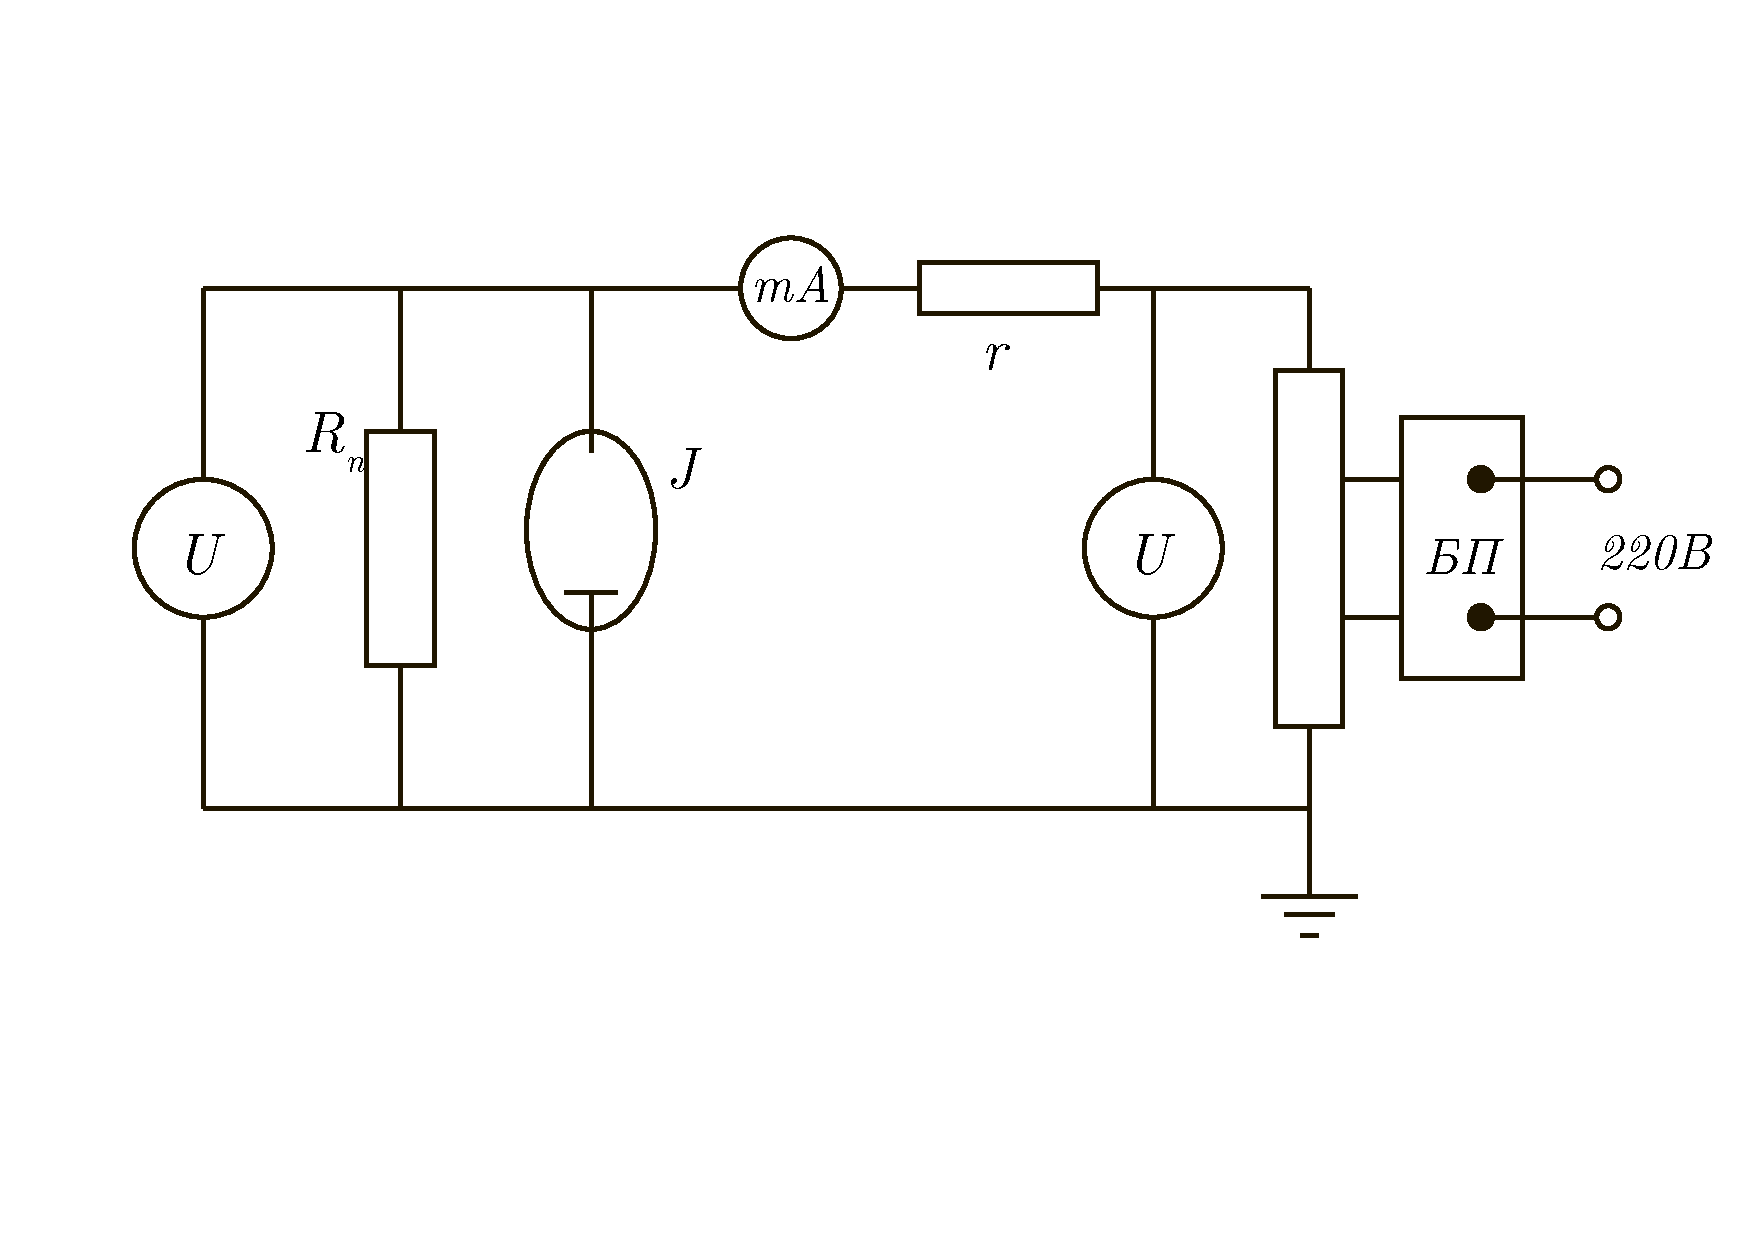
\includegraphics[scale=0.4]{Graph8.pdf}
		\caption{Простейшая схема включения стабиловольта}
		\label{fig:Graph8}
	\end{figure}
	\begin{figure}[h]
		\centering
		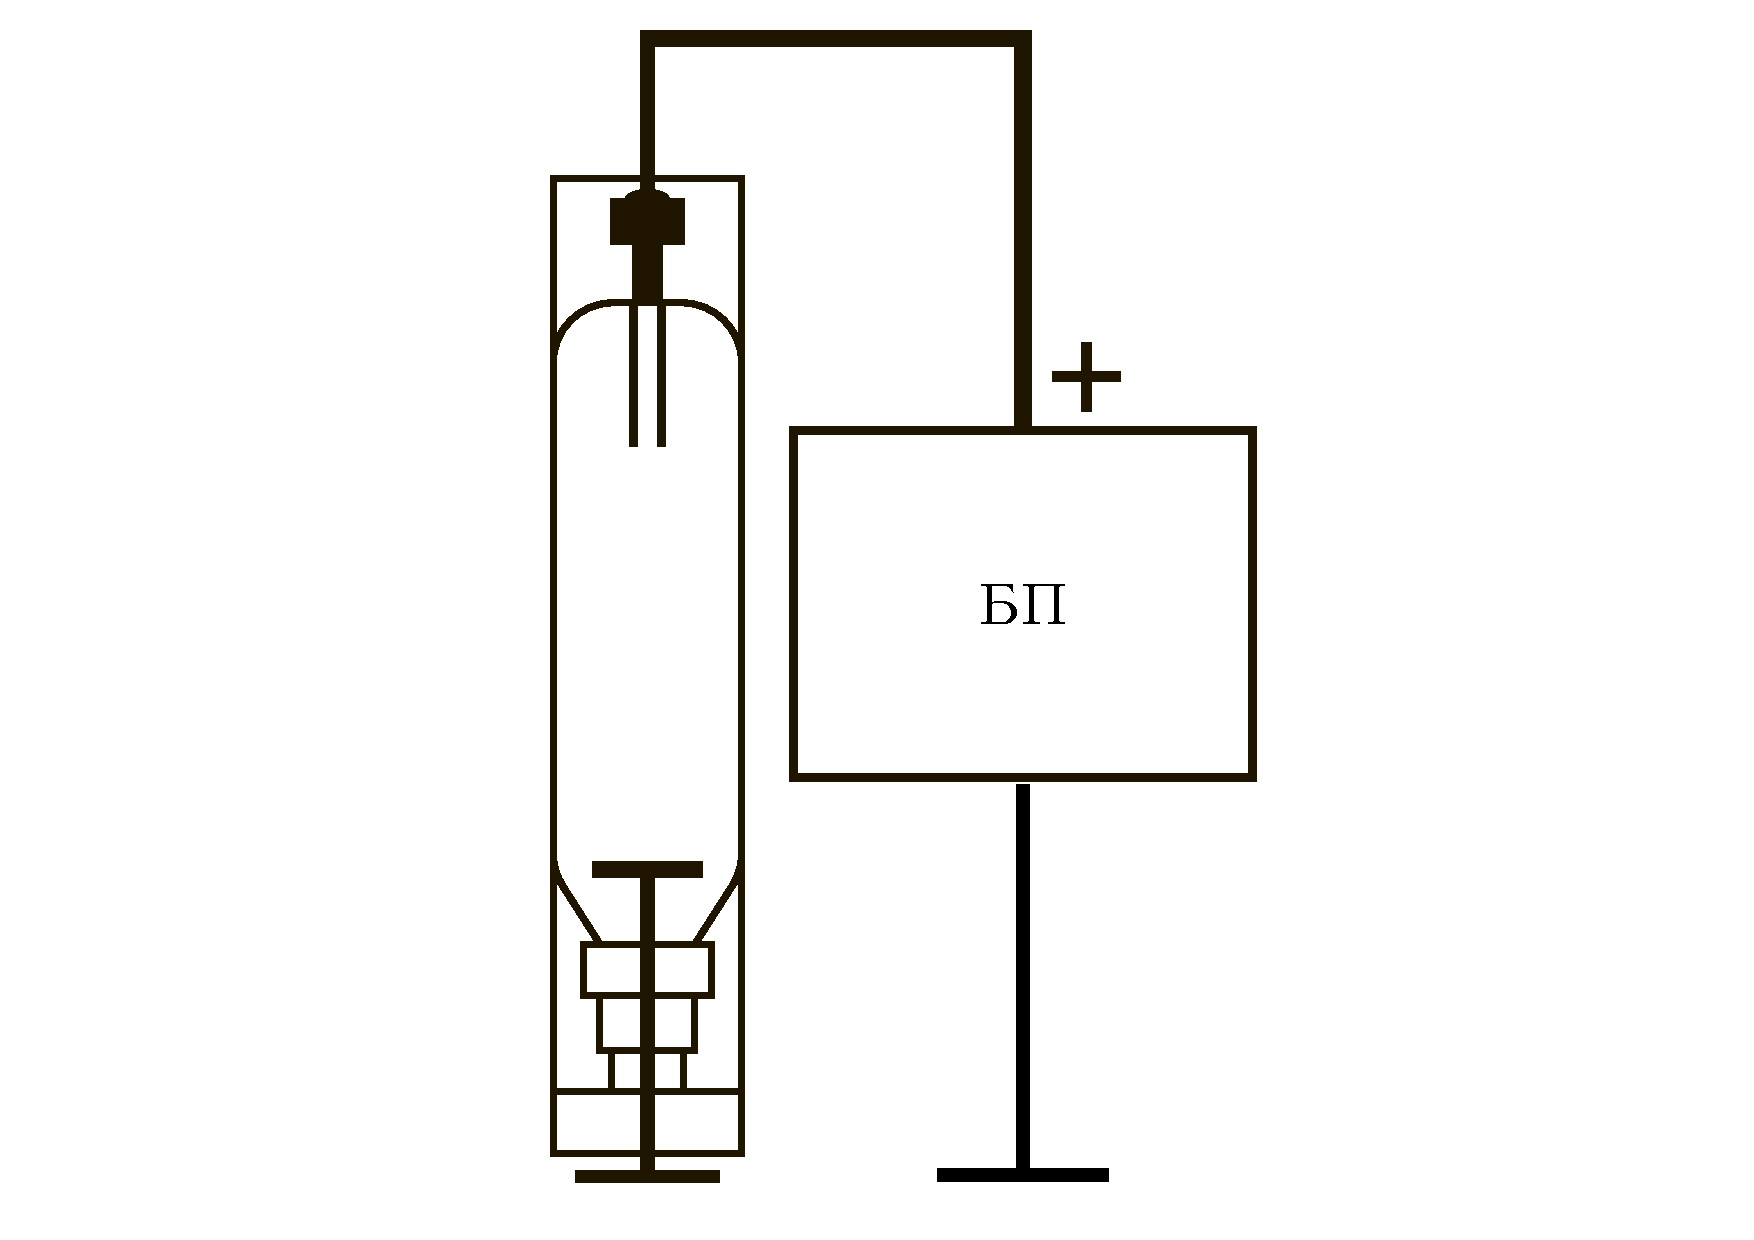
\includegraphics[scale=0.4]{Graph9.pdf}
		\caption{Рабочая схема включения стабиловольта}
		\label{fig:Graph9}
	\end{figure}
	\begin{figure}[h]
		\centering
		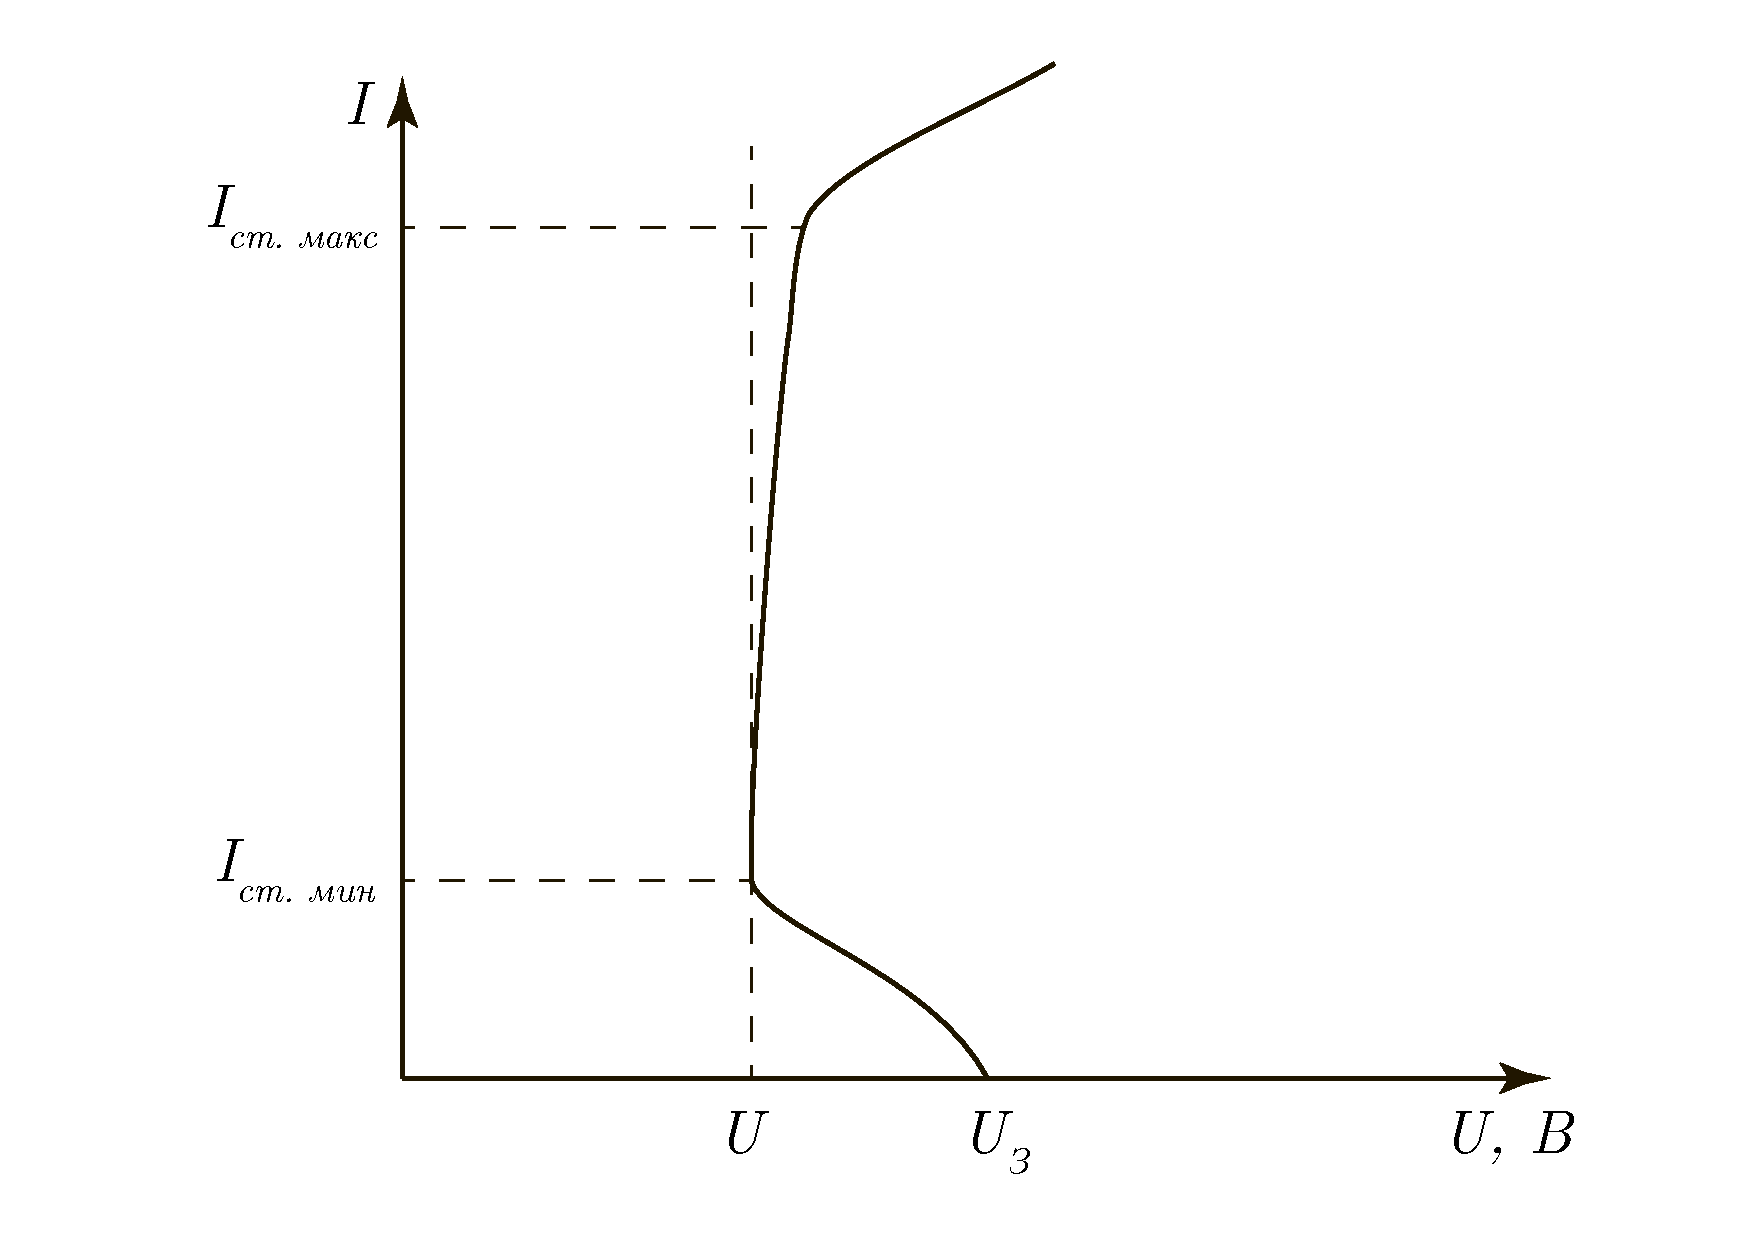
\includegraphics[scale=0.4]{Graph10.pdf}
		\caption{Вольт-амперная характеристика стабиловольта}
		\label{fig:Graph10}
	\end{figure}
	Уравнения Кирхгофа (без учета сопротивления измерительных приборов) имеют следующий вид:
	\begin{equation}
		I_0=I+I_\text{н},\quad
		U_\text{вх}=I_0r+U
	\end{equation}
	\par
	Рассмотрим, как происходит стабилизация напряжения в схеме. При увеличении входного напряжения $U_\text{вх}$ увеличится ток $I_0$ через внешнее сопротивление $r$, что вызовет увеличение падения напряжения на нем, при этом напряжение на стабиловольте и нагрузочном сопротивлении может остаться неизменным. Увеличение общего тока $I_0$ вызовет лишь увеличение тока через стабиловольт $I$. Это произойдет, если в промежутке между электродами сохраняется тлеющий разряд с нормальным катодным падением потенциала. В этом случае напряжение на стабиловольте (и на нагрузке) остается постоянным, а ток через стабиловольт может изменяться в прделах $I_\text{ст. мин}$—$I_\text{ст. макс}$. Если же ток через стабиловольт станет больше тока $I_\text{ст. макс}$, тлеющий разряд может перейти в режим аномального тлеющего разряда или в дуговой разряд, и стабилизация нарушится. Это может иметь место при относительно малом $r$ или большом увеличении входного напряжения $U_\text{вх}$.\par
	При уменьшении входного напряжения $U_\text{вх}$ ток через сопротивление $r$ и стабиловольт уменьшится, а ток через нагрузочное сопротивление и напряжение на нем останутся неизменными до тех пор, пока ток через стабиловольт не станет меньше тока $I_\text{ст. мин.}$.\par
	Таким образом, при колебаниях напряжения $U_\text{вх}$ будет меняться распределение тока между нагрузкой и стабиловольтом, а их сумма, равная $I_0$, будет меняться в зависимости от $U_\text{вх}$. Практически полагают ток нагрузки, равный примерно одной трети тока $I_\text{ст. макс}$.\par
	Важнейшие требования, предъявляемые к стабиловольтам:\par
	\begin{enumerate}
		\item Дифференциальное сопротивление разрядного промежутка $R_i$:
		\begin{equation}
			R_i=\frac{dU}{dI}
		\end{equation}
		должно быть как можно меньшим;
		\item Изменения номинальных величин $U$ и $R_i$ в зависимости от окружающей температуры должны быть возможно меньшими.
	\end{enumerate}
	Важной величиной, характеризующей работу стабиловольта в схеме, является \textbf{коэффициент стабилизации}. Он определяет как отношение относительного колебания напряжения на входе к относительному колебанию напряжения на выходе:
	\begin{equation}
		K=\frac{dU_\text{вх}/U_\text{вх}}{dU/U}=\frac{dU_\text{вх}}{dU}\cdot\frac{U}{U_\text{вх}}
	\end{equation}\par
	Используя приведенное выше уравнение Кирхгофа, получаем
	\begin{equation}
		K=\frac{1+\frac{r}{R_i}+\frac{r}{R_\text{н}}}{1+\frac{r}{R_C}+\frac{1}{R_\text{н}}}
	\end{equation}
	где $R_C=\frac{U}{I}$ — статистическое сопротивление стабиловольта, рассматриваемого в качестве нагрузки для источника напряжения.\par
	Учитывая, что в реальных случаях $R_i\ll r$ и $R_i\ll R_\text{н}$ (например, обычно $R_1=10-200$ Ом, а значения $r$ и $R_\text{н}$ составляют тысячи и десятки тысяч Ом), получаем
	\begin{equation}
		K=\frac{\frac{1}{R_i}}{\frac{1}{r}+\frac{1}{R_\text{н}}+\frac{1}{R_c}}
	\end{equation}
	\par
	Коэффициент стабилизации должен быть возможно большим. Это достигается следующим образом:
	\begin{enumerate}
		\item уменьшением $R_i$, что соответствует более вертикальной вольт-амперной характеристике стабиловольта;
		\item увеличением балластного сопротивления $r$, что связано с ростом напряжения питания $U_\text{вх}$ и потерь энергии в сопротивлении $r$, вследствие чего этот способ ограничен;
		\item увеличением статического сопротивления стабиловольта путем уменьшения тока через него. Для увеличения коэффициента стабилизации $K$ желательно работать с малыми токами через стабилизатор напряжения. Предел такому способу увеличения $K$ определяется величиной минимального тока разряда, при которой еще возможна стабилизация;
		\item увеличением сопротивленим нагрузки $R_\text{н}$. Наибольшая величина коэффициента получается при $R_\text{н}\rightarrow\infty$, т.е. в режиме холостого хода.
	\end{enumerate}
\end{document}